\chapter{Receiver Operating Characteristic Curves}
\label{ch:roc-curves}\index{ROC curves}

\section{Introduction}
\noindent A Receiver Operating Characteristic (ROC) curve is a graphical plot which presents the performance of a binary classifier when the discrimination cut-off, or threshold\index{roc-curves!threshold}, is varied. The ROC curves and associated analysis, such as area under the curve, comparing multiple ROC curves and finding an optimal threshold, have proved very useful analysis tools in many fields of research such as medical diagnosis and disease management. They have been found to be a more appropriate technique for evaluating diagnostic and predictive accuracy.

Essentially for creating and plotting the ROC curve one needs to compute the true positive rate (TPR)\index{roc-curves!true positive rate} and the false positive rate (FPR)\index{roc-curves!false positive rate} at various threshold settings and plot them in a dimensional space. In machine learning the TPR is referred to as the sensitivity\index{roc-curves!sensitivity} or recall which measures the proportion of actual positives that are correctly classified. The true negative rate (TNR)\index{roc-curves!true negative rate}, or specificity\index{roc-curves!specificity}, measures the proportion of actual negatives that are correctly identified as such. These measures can be easily summarised in Table 1 below. ROC is an evaluation procedure based on the sensitivity-specificity pair of indices.

\begin{fullwidth}
	\begin{table}[]
		\begin{tabular}{linewidth}{|l|cc|ll|}
			\hline
			\multicolumn{1}{|c|}{\textbf{Predicted Class}} & \multicolumn{2}{c|}{\textbf{True Class}}                                                                              &              &                       \\ \hline
			Yes / 1 / Positive                             & True Positives                                            & \begin{tabular}[c]{@{}c@{}}False\\ Positives\end{tabular} & TPR = TP / P & Sensitivity = TPR     \\
			No / 0 / Negative                              & \begin{tabular}[c]{@{}c@{}}False\\ Negatives\end{tabular} & True Negatives                                            & FPR = FP / N & Specificity = 1 - FPR \\ \hline
			& \textbf{P}                                                & \textbf{N}                                                &              &                       \\ \hline
		\end{tabular}
		\caption{\label{tab:sens-spec}Sensitivity and specificity}
	\end{table}
\end{fullwidth}

Consider a diagnostic test that seeks to determine whether a person has a certain disease or not. The two-class predictor yields an outcome that is labelled either positive or negative. From table 1 there are four possible outcomes from the discrete classifier: true positive or true negative if the outcome matches the actual class, false positive if the person is incorrectly classified as sick, and false negative if the person is incorrectly classified as healthy. If the test is extended to a larger sample then given a classifier and a set of instances, a 2x2 contingency table\index{roc-curves!contingency table}, or confusion matrix\index{roc-curves!confusion matrix}, can be constructed for the classifier with values for the four possible outcomes, say, sensitivity of 0.8 and specificity 0.6. Consider extending the test further to six classifiers where the same metrics are extracted from the outcomes of these classifiers. One ends up with six sensitivity-specificity pairs which are represented as points on an ROC curve as illustrated in figure 1 (adopted from \citet{fawcett2006introroc}). A to F are sensitivity-specificity pairs representing the six classifiers used in the hypothetical test. TPR (sensitivity) is plotted on the y-axis and FPR (or 1 – specificity) on x-axis. This plot depicts the relative trade-offs between true positives and false positives. The higher the sensitivity the more beneficial and trustworthy the classifier is, so TPR is a measure of the classifier's benefits. A low specificity value represents a costly classifier, so FPR is synonymous with a classifier's cost. Thus the best predictor is the one that maximises the benefits and minimises the costs. 

\begin{marginfigure}
	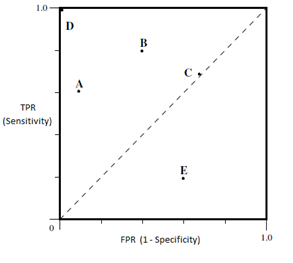
\includegraphics{roc_curves/Figure1.png}
	\caption{Basic ROC plot with five classifiers.}
	\label{fig:classifiers-roc}
\end{marginfigure}

\section{Evaluating Classifiers} \index{roc curves!evaluating classifiers}
Classifier C lies on the diagonal line from (0,0) to (1,1) of the ROC plot which represents a test that cannot distinguish between diseased and non-diseased states. Its TPR equals FPR. This means that classifier C is merely guessing the labels randomly. It is as accurate as predicting heads or tails in a coin toss. The diagonal line often serves as a benchmark for judging how well (or bad) a test performs. E and F lie on the right-hand side of the diagonal line with relatively low sensitivity and specificity metrics compared to the others. In general points on this side of the ROC plot are considered worthless (or costly) classifiers.

Classifiers A, B and D are considered better predictors from the group since they lie on the left-hand side of the diagonal line with high TPR and low FPR. D is clearly the best predictor in this case because it is the closest to the top left-hand corner of the graph. The perfect predictor would yield 100\% sensitivity and 100\% specificity with zero false positives and zero false negatives, that is, zero cost, although this is realistically very difficult to achieve. In this way the ROC plot provides an easy comparison of classifiers and leads to choosing the one that is closest to (0,1) and furthest from the diagonal line.

Consider now a continuous random variable $X$ denoting the width in millimetres of metal pipes from an automated production line is normally distributed. An inspection test might measure the diameter of the pipes and classify a pipe as defective if the width is above a certain value. Thus given a threshold width $w$, the instance is labelled defective if the continuous random variable $X$ is greater than $w$ and non-defective otherwise. As shown in figure 2 (left), one can idealise curves for both number of positive and negative results of the test. Since the test does not distinguish good pipes from defective pipes with 100\% accuracy, the distributions overlap. The overlap area indicates where the test cannot distinguish between the two classes. In practice, one chooses a cut-off (or threshold) above which the test is considered normal. Different cut-off points are used in different situations in order to minimise one of the erroneous types of the test result. The sensitivity and specificity of a classifier system depends on the particular confidence threshold that the system is using and changes inversely as the confidence threshold is changed. If the confidence threshold is made less strict, then sensitivity will increase due to more instances being classified as true positives. However, specificity will decrease because more false positives will appear. TPR and FPR increase or decrease simultaneously as the confidence interval\index{roc curves!confidence interval} threshold is changed. By repeating the experiment with adjusted thresholds, different value pairs are obtained leading to different positioning in the ROC space. 

The classifier that is able to increase the rate of detection while keeping the false alarm rate low is considered a good classifier. Figure 2 (right) shows the ROC curves with different thresholds. As the ROC curve gets closer to the top left hand of the graph the more optimal the threshold and the better the classifier's ability to discriminate between the classes.

\begin{figure}
	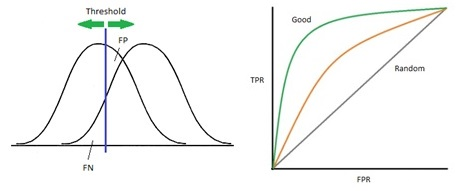
\includegraphics{roc_curves/Figure2.png}
	\caption{Left: Overlapping distributions with threshold. Right: ROC curves resulting from different thresholds.}
	\label{fig:roc-curves}
\end{figure}

\section{Area Under Curve} \index{roc-curves!area under curve}
The most common condition for choosing the optimal parameterisation is to maximise the area under the curve, AUC for short. The AUC, defined as $\int_{0}^{1} ROC(t) dt$, is a widely used measure of performance of supervised classification rules. It is a measure of the usefulness, or rather the discriminatory ability, of a test in general where the greater the area the more discriminative\index{roc-curves!discriminative} the test is in a given situation. A model or test with perfect discriminatory ability will have an AUC of, or very close to, 1.0, while a model unable to distinguish between individuals with or without the chosen outcome will have an AUC value of 0.5. 

\begin{marginfigure}
	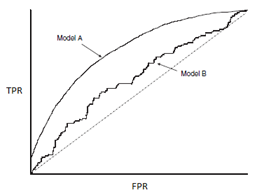
\includegraphics{roc_curves/Figure3.png}
	\caption{A comparison of two AUC curves.}
	\label{fig:two-curves}
\end{marginfigure}

However, the true value of AUC comes when comparing two or more models or tests by reducing the ROC to a single scalar value representing the expected performance of the models. Figure 3 (adopted from \citep{linden2006diagpreddismgmt}) provides a comparison between two predictive models. Model A is both statistically and visually better at identifying individuals with and without the outcome than Model B since the AUC is bigger. Therefore, if a choice was to be made between selecting one of the models, Model A would be the choice.

AUC is a desirable measure because (1) it is scale-invariant\index{roc-curves!scale invariant}: it measures how well predictions are ranked rather than their absolute values; (2) AUC is classification-threshold-invariant\index{roc-curves!classification threshold invariant}: it measures the quality of the model’s predictions irrespective of the classification threshold chosen.

\section{Multi-class ROC} \index{roc-curves!multi-class roc}
ROC curves are typically used in binary classification problems but what about multi-class problems? In order to extend ROC analysis to multi-class or multi-label classification, it is necessary to binarise the output. A multi-class problem introduces the issue of combining pairwise discriminability values. One approach introduced by \citet{provost2003treeind} was to generate each class reference ROC curve, in turn measure the AUC, then assuming the AUCs are weighted by the reference class’s prevalence in the data. Specifically, 

\begin{equation}\label{eq:multi-class}
$AUC_{total} = \sum AUC(c_{i}).p(c_{i})$ 
\end{equation}

where $c_{i}\in C$ the set of all thresholds and $p$ is the probability of class membership.

The disadvantage with this method is that the class reference ROC is sensitive to class distributions and error costs, so is the formulation of $AUC_{total}$.

To overcome this problem \citet{hand2001aucmulticlass} suggested a derivation that is based on the fact that the classifier will rank a randomly chosen positive instance higher than a randomly chosen negative instance. From this probabilistic form, they derived a formulation that measures the unweighted pairwise discriminability of classes. While this formulation is well justified and is insensitive to changes in the class distribution, they found no easy way to visualise the surface whose area is being calculated.

Thanks to its close relationship with yet another widespread Wilcoxon statistic (\citep{hanley1982useauc}), AUC methods for AUC-based analyses are well developed and widely used. However one of the major practical drawbacks of the AUC as an index of diagnostic performance\index{roc-curves!diagnostic performance} is that it summarises the entire ROC curve including the regions that are frequently not relevant to practical applications, such as regions with low level of specificity, according to \citet{ma2013paucdiagperf}. To alleviate this deficiency while benefiting from some of the advantageous properties of the area under the ROC curve, one can use a partial area under the curve (pAUC for short), which summarizes a portion of the curve over the prespecified range of interest. A number of approaches have been developed for pAUC-based analysis (\citep{dodd2003pauc,he2010nonparagenomic,mcclish1989paucanal,zhang2002nonparpaucapp}). However, \citet{ma2013paucdiagperf} argue that the same features that increase the practical relevance of the pAUC introduce some difficulty to resolve issues related to arbitrariness of specifying the range of interest. 

\begin{marginfigure}
	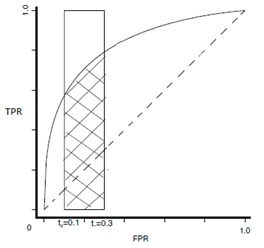
\includegraphics{roc_curves/Figure4.png}
	\caption{Illustration of an ROC curve and its partial AUC with $t_{0}$ = 0.1 and $t_{1}$ = 0.3.}
	\label{fig:partial-auc}
\end{marginfigure}

\section{Partial AUC} \index{roc-curves!partial area under curve}
\citet{dodd2003pauc} claim that in population screening, in order to avoid high monetary costs the region of the curve corresponding to low false-positive rates is of primary interest. In diagnostic testing it is critical to maintain a high TPR in order not to miss detecting diseased subjects. They go on to consider a summary index for the ROC curve restricted to a clinically relevant range of false-positive rates.

Essentially the partial AUC is simply the area under the ROC curve between $t_{0}$ and $t_{1}$ (Figure 4) where the interval ($t_{0},t_{1}$) denotes the false-positive rates of interest. The partial AUC is thus the integral between $t_{0}$ and $t_{1}$ of the ROC curve function as shown in equation 2.

\begin{equation}\label{eq:partial-auc}
AUC(t_{0},t_{1}) = \int_{t_{0}}^{t_{1}} ROC(t)  dt
\end{equation}

Selecting the interval is an important practical issue but it is beyond the scope of this chapter to delve further.

\section{Applications of ROC}
ROC curves have been used by numerous authors to evaluate models and scoring systems developed for risk assessment. For example, \citet{copp2009screening} demonstrate how the use of ROC helped in demonstrating how the fish invasiveness scoring kit distinguished accurately between potentially invasive and non-invasive species of non-native freshwater fishes. ROC analysis helped in identifying an appropriate threshold score for high-risk species. \citet{heidy2010minfneginvspec} used partial under under the ROC curve as a performance criterion to assist in providing a robust predictive model for an invasive species. \citet{makowski2010scorsysinvpests} present a procedure based on Monte Carlo simulations and ROC analysis to assess and compare scoring systems for invasive species. In their methodology the process model is a stochastic model simulating the invasion process, the candidate models are the scoring systems and the metric is the area under the ROC curve.

In disease management \citet{linden2006diagpreddismgmt} introduces ROC analysis as an appropriate tool and useful tool for evaluating diagnostic and predictive accuracy.

An interesting recent paper by \citet{fung2018cnnbcancerclass} evidences how ROC curve statistics are used to evaluate Convolutional Neural Network for breast cancer classification. It compares the ROC curves generated from the classifier with other reviewed studies. The analysis of AUC helped in evaluating the superiority of the neural network to the compared methods based on experimental results conducted on real patient subjects. Another recent paper (\citep{linden2006diagpreddismgmt}) treats a deep learning method for accurately recognises an identity from seriously noisy face images. The paper discusses ROC curves with optimal thresholds to show that noise-resistant Deep Neural Network is visibly superior to some state-of-the-art feature extraction algorithms. 

Another field where ROC proves to be contributory is psychology. Correct identification of criminals by eyewitness can help to remove a dangerous criminal from society but a false identification can lead to the erroneous conviction of an innocent suspect. A 2014 paper by \citet{gronlund2014eyewitness} describes how constructing ROC curves researchers can trace out discriminability across levels of response bias for each lineup procedure. They illustrate the shortcomings of ratio-based measures and demonstrate why ROC analysis is required for evaluating the performance of a lineup procedure. In a more recent paper \citet{luby2017lineup} goes a step further and examines the application of ROC methodology to lineup data and shows that by using a log-linear analysis in conjunction with an ROC approach to eyewitness identification it is possible not only to visualise the trade-off between true positives and false positives, but also to identify which variables are interacting with one another to explain the trade-off.

\section{History}
A final note on the history of ROC. The first use of ROC curves is traced back to World War II where in conjunction with signal detection theory, it developed for the analysis of radar images. Radar operators had to decide whether a blip on the radar screen represented and enemy target, a friendly ship or just noise. Signal detection theory measures the ability of radar receiver operators to make these important distinctions. Their ability to do so was called the Receiver Operating Characteristics. The introduction of ROC analysis into the biomedical field came in the 1970s via the radiological sciences where it has been used extensively to test the ability of an observer to discriminate between healthy and diseased subjects using a given diagnostic test, as well as to compare the efficacy among the various tests available. Since then ROC analysis has been extended for use in visualising and analysing the behaviour of a broad range of diagnostic systems across many fields of science. 

